\documentclass[a4paper, 12pt]{article}

\usepackage[utf8]{inputenc}
\usepackage[russian]{babel}
\usepackage{icomma} % smart comma(spaces could be in formulas)
\usepackage{amsmath,amsfonts,amssymb,amsthm,mathtools} %AMS

\title{\centering Отчет по заданию №1 "\textbf{Метрические алгоритмы классификации}". Алгоритм k ближайших соседей}
\date{\vspace*{\fill}Кузьмин Никита, \\ cтудент 3 курса факультета ВМК \\ кафедры ММП, \\ МГУ \\ 2019, \\ Октябрь}

% Свои команды и функции
\DeclareMathOperator{\sgn}{\mathop{sgn}}

%Убирает все номера формул, на которые не ссылок в тексте:
%\mathtoolsset{showonlyrefs=true}

\usepackage{extsizes} % Возможность сделать 14 шрифт в documentclass при article
\usepackage{geometry} % Просто способ задавать поля
    \geometry{top=25mm}
    \geometry{bottom=35mm}
    \geometry{left=35mm}
    \geometry{right=20mm}


%%% Работа с картинками
\usepackage{graphicx}  % Для вставки рисунков
\graphicspath{{images/}{images2/}}  % папки с картинками
\setlength\fboxsep{3pt} % Отступ рамки \fbox{} от рисунка
\setlength\fboxrule{1pt} % Толщина линий рамки \fbox{}
\usepackage{wrapfig} % Обтекание рисунков и таблиц текстом

%%% Работа с таблицами
\usepackage{array,tabularx,tabulary,booktabs} % Дополнительная работа с таблицами
\usepackage{longtable}  % Длинные таблицы
\usepackage{multirow} % Слияние строк в таблице
   
\usepackage{fancyhdr} % Колонтитулы
    \pagestyle{fancy}
    \renewcommand{\headrulewidth}{0pt} % Толщина линейки, отчеркивающей верхний колонтитул
%    \lfoot{Нижний левый}
%    \rfoot{Нижний правый}
%    \rhead{Верхний правый}
%    \chead{Верхний в центре}
%    \lhead{Верхний левый}

\usepackage{setspace} % Интерлиньяж
%\onehalfspacing
%\doublespacing
%\singlespacing

\usepackage{hyperref}  % Гиперссылки
\usepackage[usernames,dvipsnames,svgnames,table,rgb]{xcolor}
\hypersetup{
    unicode=true,
    pdftitle={cheat_sheet}, % Заголовок
    pdfauthor={Кузьмин Никита, ММП 317},
    pdfcreator={Кузьмин Никита, ММП 317},
    colorlinks=true, % false - ссылки в рамках; true - цветные ссылки
    linkcolor=red,   % внутренние ссылки
    citecolor=green, % на библиографию
    filecolor=magenta, % на файлы
    urlcolor=blue % на URL
}

%\renewcommand{\familydefault}{\sfdefault} % Убирает засечки у шрифта

%\usepackage{multicol} % Позволяет писать текст в несколько колонок



\begin{document}
\maketitle

\section{Свой титульный лист}
\newpage
\thispagestyle{empty}
\begin{center}
    \textit{Московский Государственный Университет имени М. В. Ломоносова\\
        Факультет выислительной математики и кибернетики}
    \vspace{0.5ex}
    \vspace{30ex}
    
    Отчет по заданию №1 "\textbf{Метрические алгоритмы классификации}". Алгоритм k ближайших соседей
    
\end{center}
\vspace{13ex}
\begin{flushright}
    \noindent % Убирает красную строку
    \vfill
    \textit{Кузьмин Н. В.}
    \\
    \textit{студент кафедры ММП \\ 317 группа}
    
\end{flushright}
\begin{center}
    Октябрь,
    
    2019
\end{center}

\newpage
\section{Первый раздел}\label{razdel}
\subsection{Subsection}\label{podrazdel}
В разделе \ref{razdel} начинается документ
Подраздел \ref{podrazdel}  

\newpage
Первый абзац
$ 2 + 2 = 4$
\[2 + 3 = 5\]
$2,4$

$(2, 4)$
\begin{equation}\label{eq:mrmc}
MR=MC
\end{equation}

\eqref{eq:mrmc} на стр \pageref{eq:mrmc} ---  условие максимизации прибыли

\[\frac{1+\dfrac{4}{2}}{6} = 0,5\]

\subsection{Скобки}
плохой размер скобок:
\[(2 + \frac{9}{3})\times 5 = 25\]
хороший размер скобок:
\[\left(2 + \frac{9}{3}\right)\times 5 = 25\]

\[[2+3]\]
Обязательно ставить \ перед фигурными скобками, иначе они не отобразятся!
\[\{2+3\}\]

\subsection{Стандартные функции}

$\sin x = 5$, 
$\ln x = 5$,
$\sgn x = 1$

\subsection{Символы}\label{symbols}

$2\times 2 \ne 5$

$A \cap B,A \cup B$

\subsection{Диакритические знаки}

$\bar x =5$, $\tilde{x} = 8$

Если хотим отрицание над несколькими переменными:
\[\bar{xyz} = 1\]

Но так вышло плохо, исправим:
\[\overline{xyz} = 1\]

\[\widetilde{xywew} = 5\]

\subsection{Буквы других алфавитов}

\[tg(\alpha) = 1\]
Для больших греческих букв:
\[tg(\Phi) = 5\]
Некоторые правила написания греческих букв.
\[\epsilon\]
Эпсилон выглядит не очень привычно, изменим:
\[\varepsilon\]

\section{Формулы в несколько строк}

\subsection{Очень длинные формулы}
\begin{multline}
1+2+3+4+5+6+7 \dots + \\ + 50 + 51 + 52 + 53 + 53 + 54 + 55+ 56 + 57 + \dots + \\ + 96 + 97 + 98 + 99 + 100
\end{multline}

Несколько формулы, их выравнивание с помощью align. Нечетные \& отвечают за выравнивание внутри столбца, а четные \& за создание нового столбца
\begin{align}
2\times 2 &= 4& 6\times 8 &= 48\\
3\times 3 &= 9& a + b &= c\\
10\times 10 &= 100& \frac{1}{5} &= 0.2
\end{align}

Если не хотим нумеровать - align*:
\begin{align*}
2\times 2 &= 4& 6\times 8 &= 48\\
3\times 3 &= 9& a + b &= c\\
10\times 10 &= 100& \frac{1}{5} &= 0.2
\end{align*}

Для нумерации группы формул:
\begin{equation}
\begin{aligned}
2\times 2 &= 4& 6\times 8 &= 48\\
3\times 3 &= 9& a + b &= c\\
10\times 10 &= 100& \frac{1}{5} &= 0.2
\end{aligned}
\end{equation}


\subsection{Системы уравнений}
Обычная:
\[\left\{
\begin{aligned}
2\times 2 &= 4& 6\times 8 &= 48\\
3\times 3 &= 9& a + b &= c\\
10\times 10 &= 100& \frac{1}{5} &= 0.2
\end{aligned}\right.
\]
С условиями:
\[
|x| = \begin{cases}
x, &\text{if } x \ge 0 \\
-x, &\text{if } x < 0
\end{cases}
\]

\section{Матрицы}
Матрица в круглых скобках:
\[
\begin{pmatrix}
a_{11} & a_{12} & a_{13}\\
a_{21} & a_{22} & a_{23}\\
a_{31} & a_{32} & a_{33}\\
\end{pmatrix}
\]
Определитель матрицы:
\[
\begin{vmatrix}
a_{11} & a_{12} & a_{13}\\
a_{21} & a_{22} & a_{23}\\
a_{31} & a_{32} & a_{33}\\
\end{vmatrix}
\]
Матрица в квадратных скобках(используем tag для своей нумерации)
\[
\begin{bmatrix}
a_{11} & a_{12} & a_{13}\\
a_{21} & a_{22} & a_{23}\\
a_{31} & a_{32} & a_{33}\\
\end{bmatrix}\tag{MATRIX}
\]

\section{Кегль}
    \begin{table}[h!]
        \caption{Размеры шрифта}
        \centering
        \begin{tabular}{|c|c|}
            \hline	\verb|\tiny|      & \tiny        крошечный \\
            \hline	\verb|\scriptsize|   & \scriptsize  очень маленький\\
            \hline \verb|\footnotesize| & \footnotesize  довольно маленький \\
            \hline \verb|\small|        &  \small        маленький \\
            \hline \verb|\normalsize|   &  \normalsize  нормальный \\
            \hline \verb|\large|        &  \large       большой \\
            \hline \verb|\Large|        &  \Large       еще больше \\[5pt]
            \hline \verb|\LARGE|        &  \LARGE       очень большой \\[5pt]
            \hline \verb|\huge|         &  \huge        огромный \\[5pt]
            \hline \verb|\Huge|         &  \Huge        громадный \\ \hline
        \end{tabular}
    \end{table}

Какой-\scriptsize нибудь \Large обычный \normalsize текст.

\begin{Huge}
    А можно так,
    
    \textbf{если нужно выделить абзац}
\end{Huge}

Или {\Large вот} так

Какой-то текст \emph{c выделением  }


\section{Гиперссылки}
\url{https://msu.ru}

Сайт \href{http://msu.ru}{МГУ}

\section{Перечни}
\begin{itemize} 
    \item Это
    \item Маркированный
    \begin{itemize}
        \item Подсписок
    \end{itemize}
    \item Список
\end{itemize}
Еще один вид:\\
\begin{enumerate}
    \item А это
    \item нумерованный
    \item список
    \item[123.] Можно и так!
\end{enumerate}

\section{Картинки и Таблицы}
Картиночка:
\\
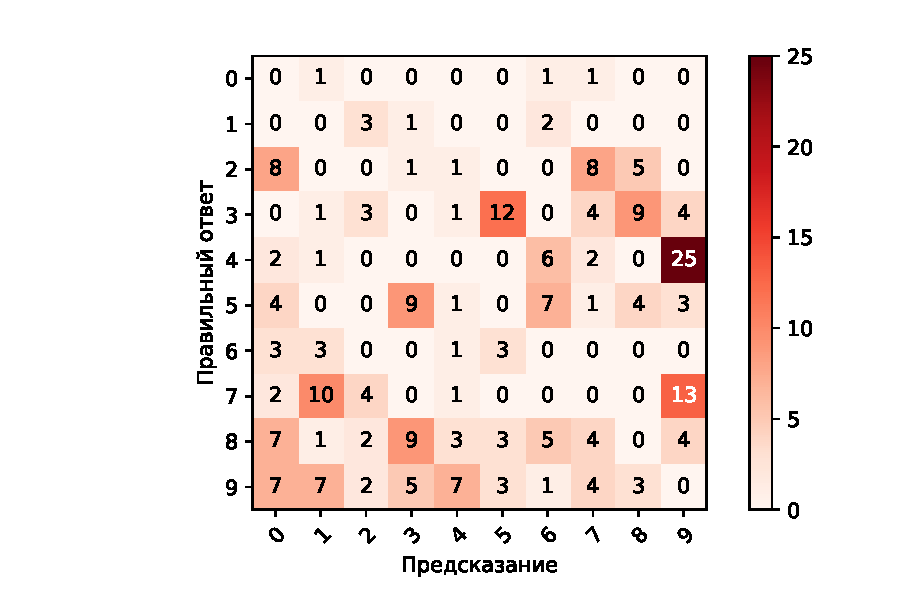
\includegraphics{../conf_matrix_experiment_4.pdf}

\begin{tabular}{c|cc}
    a & a & a
\end{tabular}

\subsection{Картинки}
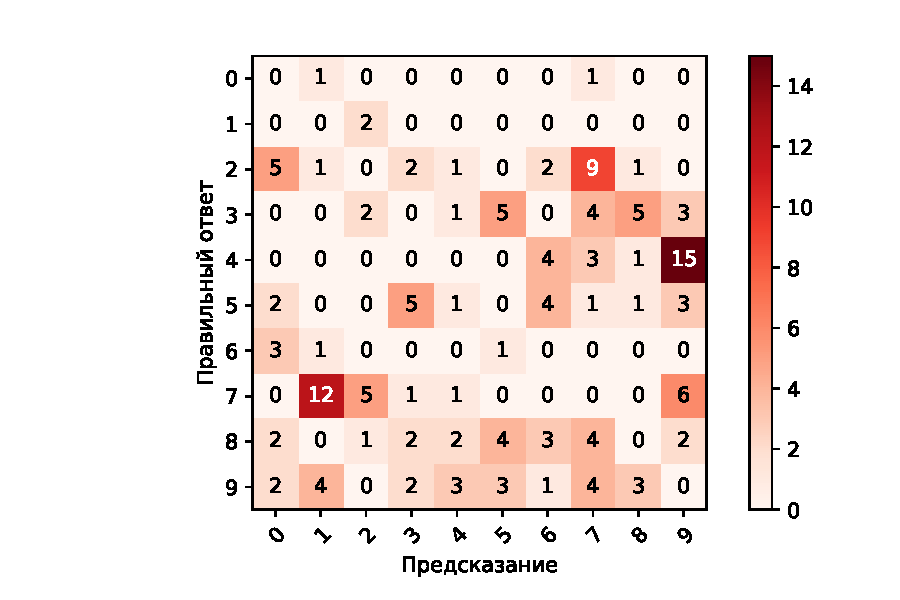
\includegraphics{../conf_matrix_experiment_5_with_full_aug_on_train.pdf}

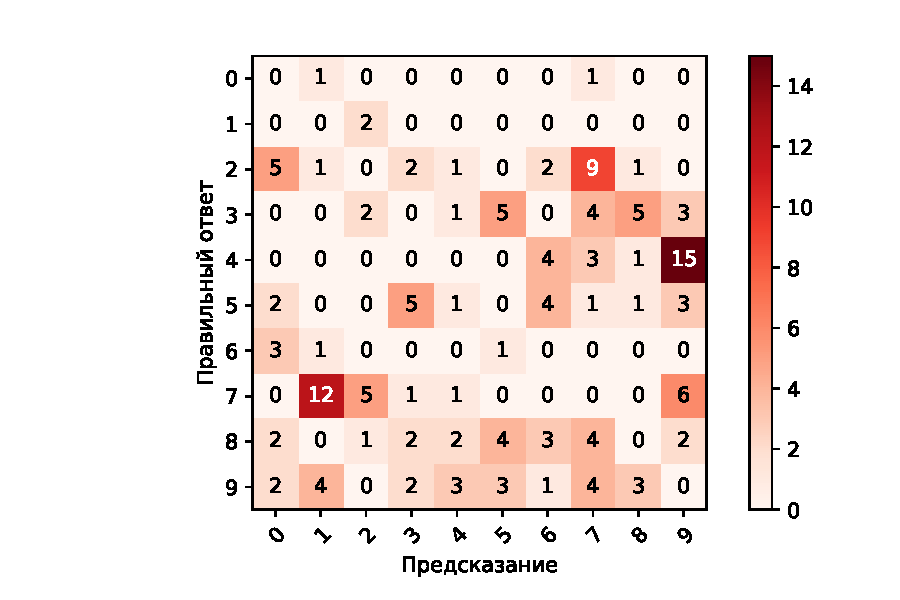
\includegraphics[scale=0.5]{../conf_matrix_experiment_5_with_full_aug_on_train.pdf}

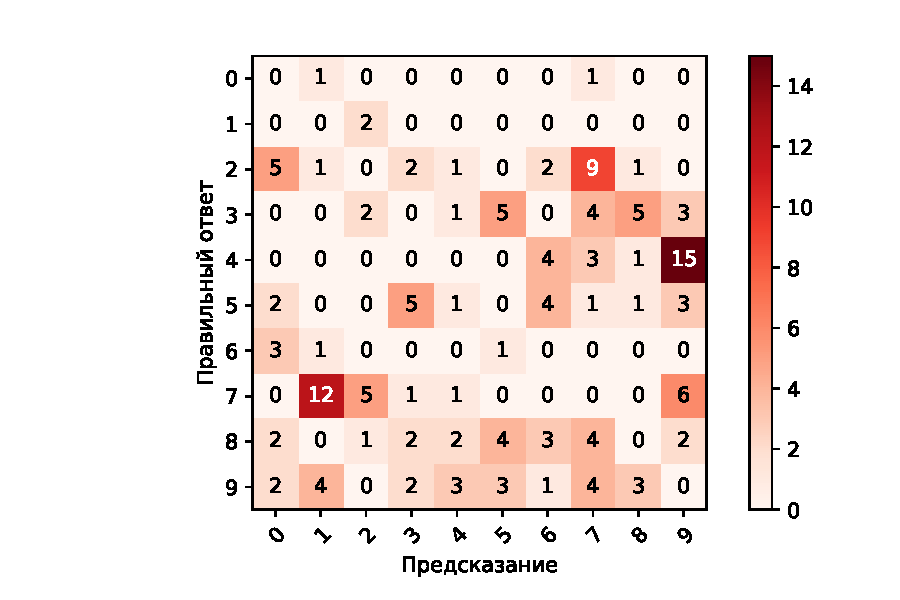
\includegraphics[width=15cm, height=8cm, keepaspectratio]{../conf_matrix_experiment_5_with_full_aug_on_train.pdf}

\begin{figure}
    \caption{Матрица ошибок}\label{confusion_matrix5}
    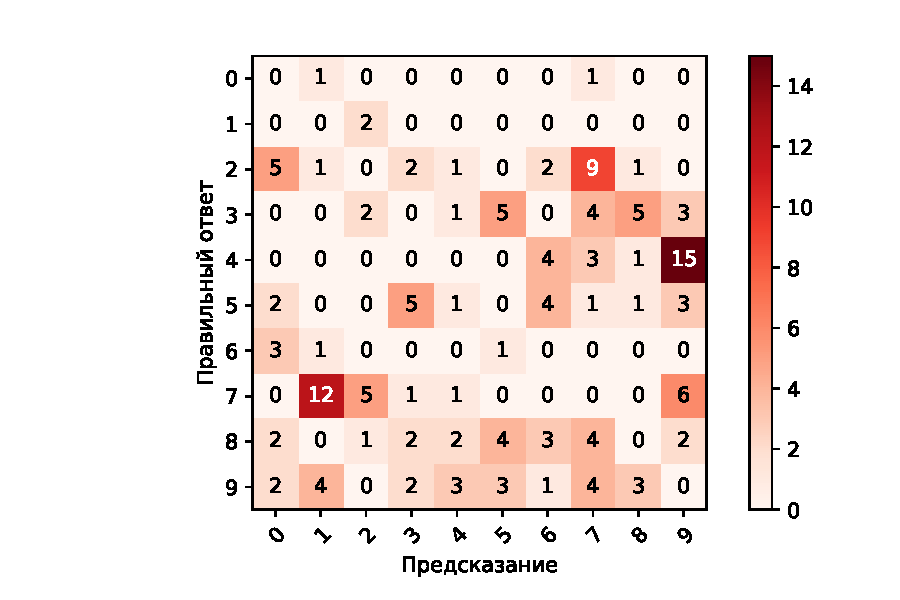
\includegraphics[width=\textwidth]{../conf_matrix_experiment_5_with_full_aug_on_train.pdf}
\end{figure}
\ref{5}

\subsection{Таблички}

\begin{tabular}{|l|c|r|}
    \hline 
    11 & 12 & 13 \\ 
    %\hline 
    5 &  6 & 7  \\ 
    \hline 
    1 & 2 & 3 \\ 
    \hline 
\end{tabular} 

Табличка, которая не выезжает за границы - \textbf{tabularx}

\begin{tabularx}{\textwidth}{X|c|X}
    \hline
    Очень длинное предложение очень очень длинное! & Очень длинное & Очень длинное предложение очень очень длинное!
\end{tabularx}

\begin{tabulary}{\textwidth}{C|J|R}
     \hline
    Очень длинное предложение очень очень длинное! & Очень длинное & Очень длинное предложение очень очень длинное!
\end{tabulary}

\section{Плавающие объекты}

Смотри таблицу \ref{tab:mytab}.

\begin{table}[h] % вставляет таблицу туда, где встречается описание её
    \begin{center}
        \caption[Заголовок для списка таблиц]{Бессмысленная таблица, зато с кучей фишек.}\label{tab:mytab}
        \begin{tabular}{|c|c|c|c||l|c|c|r|c|c|}
            \hline
            1 & 2 & 3 & 4 & 5 & 6 & 7 & 8 & 9 & 10 \\ \hline
            Первый & Второй & \multicolumn{3}{|c|}{Третий -- пятый} &   &  & Восьмой &   &  \\  % слияние столбцов
            \cline{1-7} \cline{9-10}
            1 & 2 & 3 & 4 & 5 & 6 & 7 & 8 & 9 & 10 \\ \hline \hline
            1 & 2 & 3 & 4 & 5 & 6 & 7 & 8 & 9 & 10 \\ \hline
            \multirow{3}{*}{Три строки}  & 2 & 3 & 4 & 5 & 6 & 7 & 8 & 9 & 10 \\ \cline{2-10}
            & 2 & 3 & 4 & 5 & 6 & 7 & 8 & 9 & 10 \\ \cline{2-10}
            & 2 & 3 & 4 & 5 & 6 & 7 & 8 & 9 & 10 \\ \hline
        \end{tabular}
    \end{center}
    %\caption{Заголовок мог быть и здесь}
\end{table}




\begin{longtable}{|c|c|c|c|}
    \caption{Заголовок большой таблицы.}\\
    \hline
    \textbf{RND1} & \textbf{RND2} & \textbf{RND3} & \textbf{RND4} \\ \hline
    \endfirsthead
    \hline
    RND1 & RND2 & RND3 & RND4 \\ \hline
    \endhead
    \hline
    \multicolumn{4}{r}{продолжение следует\ldots} \
    \endfoot
    \hline
    \endlastfoot
    
    0,576745371 & 0,435853468 & 0,36384912 & 0,299047979 \\ 
    0,064795364 & 0,028454613 & 0,751312059 & 0,693972684 \\
    0,263563971 & 0,367508634 & 0,075536384 & 0,337780707 \\
    0,957583964 & 0,431948588 & 0,938522377 & 0,464307785 \\
    0,815740484 & 0,123129806 & 0,883432767 & 0,760983283 \\
    0,445062335 & 0,157424268 & 0,883442259 & 0,300596338 \\
    0,187159669 & 0,728663343 & 0,637199982 & 0,765684528 \\
    0,41009848 & 0,457031472 & 0,142858106 & 0,602946607 \\
    0,43315663 & 0,26058316 & 0,611667007 & 0,400328185 \\
    0,824086963 & 0,27304335 & 0,244565296 & 0,219675484 \\
    0,109578811 & 0,278478018 & 0,242519359 & 0,414669471 \\
    0,220778432 & 0,938106645 & 0,502630894 & 0,910760406 \\
    0,905239004 & 0,017835419 & 0,429423867 & 0,299079986 \\
    0,604679988 & 0,784786124 & 0,86825382 & 0,003631105 \\
    0,725883239 & 0,273875543 & 0,843605984 & 0,607743466 \\
    0,555736787 & 0,019487901 & 0,342950631 & 0,537183422 \\
    0,309374962 & 0,44331087 & 0,749656403 & 0,966836051 \\
    0,274332831 & 0,740197878 & 0,865450742 & 0,792816484 \\
    0,968626843 & 0,580215733 & 0,706427331 & 0,879562225 \\
    0,281344607 & 0,51362826 & 0,7998827 & 0,270290356 \\
    0,885143961 & 0,989455756 & 0,235591368 & 0,693434397 \\
    0,505067377 & 0,127308502 & 0,614625825 & 0,277375342 \\
    0,663594497 & 0,023550761 & 0,670822594 & 0,302446663 \\
    0,094723947 & 0,091199224 & 0,841117852 & 0,617394243 \\
    0,490246305 & 0,761569651 & 0,973576975 & 0,51597127 \\
    0,631301873 & 0,155944248 & 0,319958965 & 0,198643097 \\
    0,853761692 & 0,993889567 & 0,105045533 & 0,837805396 \\
    0,149834425 & 0,316419619 & 0,387770251 & 0,552013475 \\
    0,269182006 & 0,721020214 & 0,484218147 & 0,552132834 \\
    0,668632873 & 0,699511389 & 0,278877959 & 0,021775345 \\
    0,62638369 & 0,737702261 & 0,696351048 & 0,256427487 \\
    0,922563692 & 0,629514529 & 0,789891184 & 0,019748079 \\
    0,366649518 & 0,882085214 & 0,805771543 & 0,461659364 \\
    0,178967822 & 0,400706498 & 0,313063544 & 0,425676173 \\
    0,328582166 & 0,124008134 & 0,177734655 & 0,653821253 \\
    0,318628436 & 0,924056157 & 0,005170407 & 0,09988244 \\
    0,1523348 & 0,686022531 & 0,877786704 & 0,230997696 \\
    0,160048577 & 0,475334591 & 0,118018156 & 0,720594848 \\
    0,502602506 & 0,898504748 & 0,103602236 & 0,289059862 \\
    0,185262766 & 0,640333509 & 0,980932923 & 0,424269289 \\
    0,63740761 & 0,665837647 & 0,256564927 & 0,796877433 \\
    0,326795292 & 0,863892719 & 0,19537989 & 0,410369904 \\
    0,377332846 & 0,61459335 & 0,158101373 & 0,100684292 \\
    0,540188499 & 0,911708617 & 0,077277867 & 0,108818241 \\
    0,485200234 & 0,692007154 & 0,012528805 & 0,364692863 \\
    0,435947515 & 0,555444136 & 0,410076838 & 0,973027822 \\
    0,423053661 & 0,502696027 & 0,500150945 & 0,209929767 \\
    0,146604488 & 0,318962234 & 0,535025906 & 0,25597358 \\
    0,252933039 & 0,897587117 & 0,961039174 & 0,238301151 \\
    0,798559806 & 0,885674601 & 0,451623639 & 0,903044881 \\
    0,467795852 & 0,398491485 & 0,09863235 & 0,110588673 \\
    0,932456386 & 0,679931054 & 0,499049066 & 0,419347908 \\
    0,806742814 & 0,998944815 & 0,730738513 & 0,207088322 \\
    0,524028453 & 0,251332909 & 0,711910448 & 0,243583774 \\
    0,037417208 & 0,333822686 & 0,276647434 & 0,882818666 \\
    0,358649112 & 0,534662608 & 0,726203191 & 0,041117785 \\
    0,141309914 & 0,36643456 & 0,552053605 & 0,956487966 \\
    0,53808496 & 0,939874695 & 0,186724749 & 0,690302117 \\
    0,052101497 & 0,887611776 & 0,677925016 & 0,622234766 \\
    0,553154653 & 0,040281685 & 0,504952332 & 0,097544063 \\
    0,732288281 & 0,658739311 & 0,883348524 & 0,144957902 \\
    0,288649747 & 0,517727905 & 0,639432157 & 0,456739615 \\
    0,293369191 & 0,138002629 & 0,154228354 & 0,133189564 \\
    0,693221668 & 0,246693033 & 0,465542044 & 0,978720597 \\
    0,135587928 & 0,15068455 & 0,825417066 & 0,885949167 \\
    0,676052335 & 0,253724745 & 0,219361854 & 0,808580891 \\
    0,582461065 & 0,554730526 & 0,476287005 & 0,268673107 \\
    0,238129516 & 0,090469211 & 0,525167086 & 0,59620778 \\
    0,769704124 & 0,27036399 & 0,888763617 & 0,089602751 \\
    0,548435183 & 0,357753532 & 0,858061896 & 0,465681708 \\
    0,702731358 & 0,856923488 & 0,058935386 & 0,675796794 \\
    0,338117119 & 0,622858325 & 0,461848295 & 0,94572588 \\
    0,606619551 & 0,999527337 & 0,361750308 & 0,673771858 \\
    0,221137745 & 0,719189979 & 0,624447286 & 0,59032258 \\
    0,239784727 & 0,636404041 & 0,841898027 & 0,844823258 \\
    0,800614467 & 0,368896918 & 0,994129014 & 0,291457496 \\
    0,681757552 & 0,019367985 & 0,417601531 & 0,649347809 \\
    0,28051889 & 0,061635488 & 0,914332594 & 0,331713964 \\
    0,657743996 & 0,983965656 & 0,818946725 & 0,36394332 \\
    0,543479307 & 0,169289586 & 0,483196672 & 0,985172369 \\
    0,145081556 & 0,892455096 & 0,190462767 & 0,824433551 \\
    0,196973955 & 0,995308839 & 0,879891823 & 0,845636911 \\
    0,904947195 & 0,593928658 & 0,403422613 & 0,076252813 \\
    0,269580321 & 0,740772576 & 0,182364329 & 0,695081896 \\
    0,293711052 & 0,351494187 & 0,331350034 & 0,62158188 \\
    0,69779066 & 0,019424915 & 0,657473072 & 0,783698296 \\
    0,14204222 & 0,817006985 & 0,669234791 & 0,728306309 \\
    0,38941124 & 0,807135743 & 0,702842593 & 0,382494957 \\
    0,203543688 & 0,969191131 & 0,822881425 & 0,212473701 \\
    0,826623142 & 0,181291269 & 0,054701556 & 0,386442059 \\
    0,541365118 & 0,573617788 & 0,650112336 & 0,930417614 \\
    0,277453725 & 0,382833978 & 0,395547164 & 0,785051981 \\
    0,078149646 & 0,115526198 & 0,417197235 & 0,894812516 \\
    0,772854891 & 0,698024923 & 0,504995217 & 0,492422679 \\
    0,592288285 & 0,153957871 & 0,348784682 & 0,523821625 \\
    0,618156868 & 0,841905787 & 0,038053593 & 0,861496223 \\
    0,76387049 & 0,652733723 & 0,034948244 & 0,814496925 \\
\end{longtable}

\section{Обтекание объектов текстом}
\begin{wrapfigure}{l}{0.5\linewidth}
    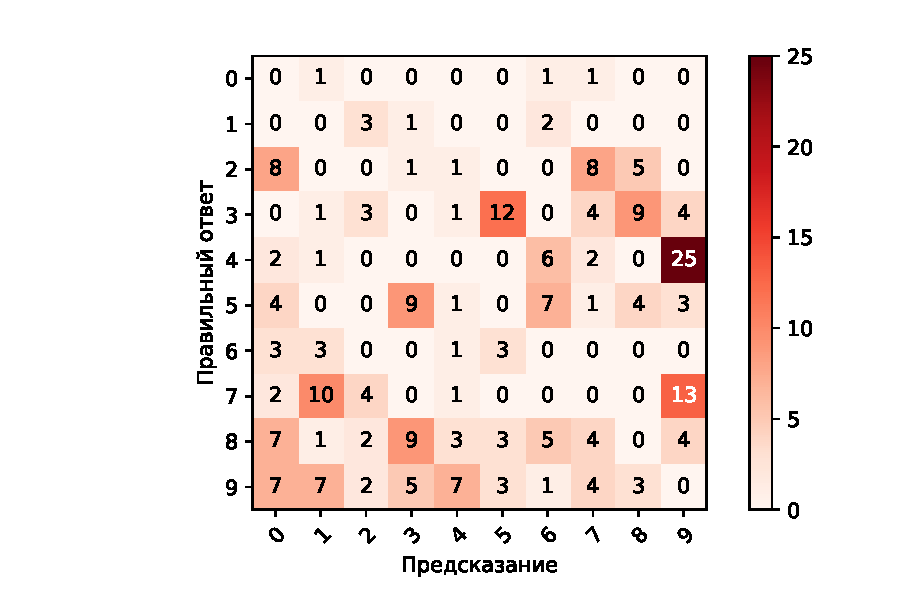
\includegraphics[width=\linewidth]{../conf_matrix_experiment_4.pdf}
    \caption{Картинка с обтеканием}
\end{wrapfigure}
Получим, что число узлов вывода равно числу классов входного набора данных.

Значения слоя вывода умножаются на веса, к ним добавляется смещение, но функция активации уже другая.

Мы хотим пометить каждый текст категорией, между собой они являются взаимоисключающими, т.к. текст не может принадлежать двум категориям одновременно. Чтобы достичь цели, вместо ReLu возьмем функцию Softmax. Она преобразует вывод для каждой категории в значение между 0 и 1, а также проверяет, что сумма всех значений равна 1. Так вывод покажет нам вероятность принадлежности текста к каждой категории:

\begin{wraptable}{r}{0.5\linewidth}
    \begin{tabular}{|c|c|c|c|c|c|}
        \hline
        Год & $P_x$ &$Q_x$ & $P_y$ & $Q_y$ & $n$\\ \hline
        2008 &  & 36 &  & 32 & — \\ \hline
        2009 & 30 & 30 & 22 & 50 & 25 \% \\ \hline
        2010 & 36 & 30 & 22 &  & 20 \% \\ \hline
        2011 & 33 & 40 & 24 & 45 & \\ \hline
    \end{tabular}
    \caption{Обтекаемая таблица}
\end{wraptable}
Вам также надо определить, сколько узлов будет содержать первый скрытый слой. Они называются признаками или нейронами, на изображении сверху каждый представлен синим кругом.

В слое ввода один узел соответствует слову из набора данных. Рассмотрим это чуть позже.

Как объяснено в этой статье, каждый узел (нейрон) умножается на вес, т.е. имеет значение веса. В ходе обучения нейронная сеть регулирует эти показатели, чтобы произвести правильные выходные данные. Сеть также добавляет смещение.

Далее в нашей архитектуре данные передаются функции активации, которая определяет окончательный вывод каждого узла. Приведем аналогию: представьте, что каждый узел — это лампа, а функция активации указывает, будет лампа гореть или нет.

Существует много видов функции активации. Используем усеченное линейное преобразование (ReLu). Эта функция определяется следующим образом:


\section{Список иллюстраций и список таблиц}

\listoffigures

\listoftables

\end{document}